\section{Blocking}
	\label{sec:blocking}
		The data produced by Monte Carlo methods are typically a finite time series of correlated data. Many results, like the energy in the variational Monte Carlo solver, are averages over a finite time, and thus vary from simulation to simulation. Estimating the error on a time average of correlated data is therefore of great importance to be able to have information about how accurate the results produced are. There are several estimators of this error, like those described in Refs. \cite{binder1984} and \cite{daniell1984}. A more effortless method, however, is the blocking method. 

		The exact origin of the blocking method is uncertain, but it is plausible that it was invented by K. Wilson \cite{Wilson1980}. It is also briefly described by Whitmer \cite{whitmer1984} and Gottlieb et al. \cite{gottlieb1986}. For a more thorough description of the method, see the article by Flyvbjerg and Petersen \cite{flyvbjerg1989}. 

		The blocking method is independent from the VMC computation, and can be used afterwards to get a more robust estimate of the variance. The basic idea lies on the correlations between all the measurements. If these are important enough, they will produce an increase in the error that needs to be taken into account. The reason behind this is related to the effective amount of measurements, if there are correlations there will be measurements that will contain less information, so these won't be as valuable as the rest and it will be as if there are \textit{less} measurements than we actually have. Obviously this is a problem, the usual identification of the error with $\sqrt{\sigma/n}$ will be overly optimistic and a correction is needed. 
		%\todo{Mer tekst om blocking}

		We introduce
		\begin{align}
			f_d=\frac{1}{n-d}\sum_{k=1}^{n-d}{\left(x_k-\bar{x}_n\right)\left(x_{k+d}-\bar{x}_n\right)},
		\end{align}
		where $f_d$ is the correlation between measurements separated by a distance of $d$. This can be used to give an actual form to the correction factor,

		\begin{align}
			\tau=1+2\sum_{d=1}^{n-1}{\frac{f_d}{var\left(x\right)}}.
		\end{align}

		This is the autocorrelation time and it relates the error with the variance,

		\begin{align}
			err^2=\frac{\tau}{n}var\left(x\right).
		\end{align}

		The inverse of the first factor is  the number of effective measurements (that are useful since they contain information),

		\begin{align}
			n_{eff}=\frac{n}{\tau}.
		\end{align}

		The expression that relates the standard deviation with this correlation time is thus

		\begin{align}
			\sigma=\sqrt{\left(\frac{1+2\tau/\Delta t}{n}\left(\bar{x^2}-\bar{x}^2\right)\right)},
		\end{align}

		where $\Delta t$ is the time between samples, commonly smaller than $\tau$. The main problem is that to compute $\tau$ a lot of time is needed, and this is not feasible in most cases.

		The solution is to use blocking, and the algorithm for it is fairly straightforward 
		\begin{itemize}
			\item Take a sequence of measured data and divide the sequence into blocks.
			\item Calculate the total mean and variance from the mean, $\bar{x}_i$, of block $i=1\dots n_{blocks}$, making sure the block-size is large enough so that sample $j$ of block $i$ is not correlated with sample $j$ of block $i+1$.
			\item A good choice for the size would be the correlation time, $\tau$. However, it is unknown. Therefore make a plot of the standard deviation $\sigma$, as a function of the block-size.
			\item When the standard deviation reaches a plateau the blocks are uncorrelated.
		\end{itemize} 
		
		With the standard deviation reaching the plateau and the blocks thus are uncorrelated, we have an approximation to the true error, in form of the covariance. In some cases the data is fairly uncorrelated, however. In cases like that there is no plateau, only a seemingly random  spread of the standard deviations with respect to block size. For an example of the two cases, see figure Fig. \ref{fig:blocking_example}.


		\begin{figure}[H]
			\begin{centering}
				\subfloat[]{\begin{centering}
					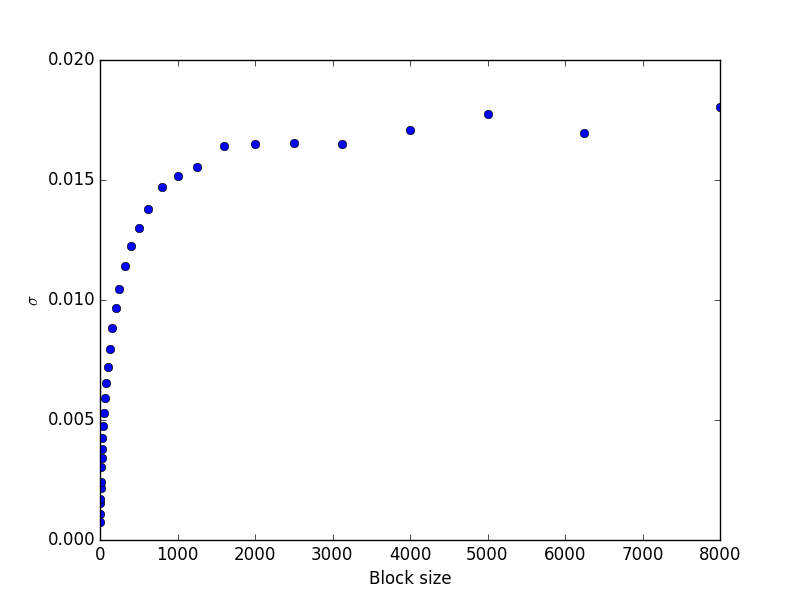
\includegraphics[width=0.5\linewidth]{content/Theory/figures/blocking_QD2_w1}
				\par\end{centering}

				}\subfloat[]{\begin{centering}
					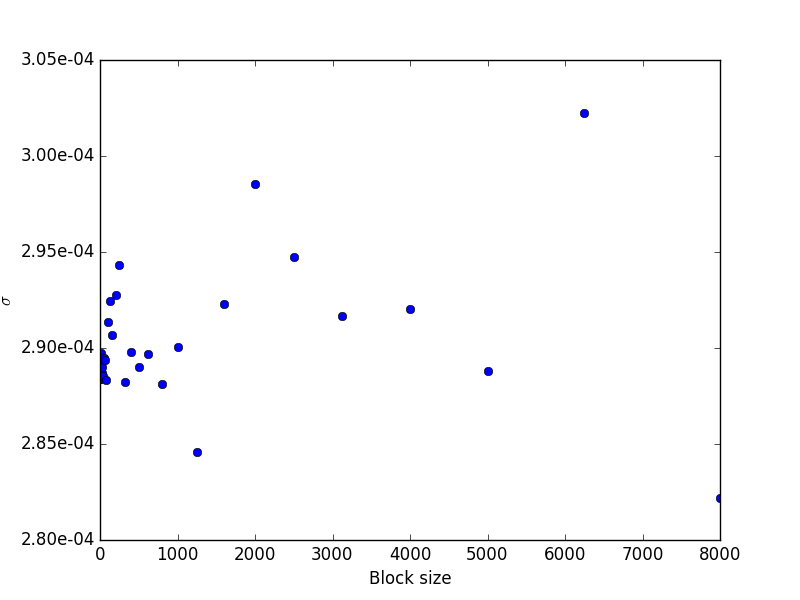
\includegraphics[width=0.5\linewidth]{content/Theory/figures/blocking_test2}
				\par\end{centering}

				}
			\par\end{centering}

			\protect\caption{\textbf{(a)}: Result from blocking of a VMC simulation of a 2-particle quantum dot in two dimensions, with frequency $\omega = 1.0$. There is a clear plateau, which means that the data is correlated, and the true error is approximately $1.6\times 10^{-2}$. \textbf{(b)}: Result from blocking of data from a Monte Carlo integration. The data is uncorrelated, resulting in no plateau and a distribution of standard deviations spread out around $2.9\times 10^{-4}$. The definite integral calculated is $\int _{0}^{\pi} \sin (x)dx= 2$, where the Monte-Carlo integrator gives the result $2.00003$, in agreement with the magnitude of error. \label{fig:blocking_example}}
		\end{figure}




